%///////////////////////////////////////////////////////////////////////////////
% <file type="public">
%
% <license>
%   See the src/README.txt file for this module for copyright and license
%   information.
% </license>
%   <description>
%     <abstract>
%       This is the Webnucleo Report describing low temperature equilibria.
%     </abstract>
%     <keywords>
%       libnuceq, report
%     </keywords>
%   </description>
%
%   <authors>
%     <current>
%       <author userid="mbradle" start_date="2010/12/23" />
%     </current>
%     <previous>
%     </previous>
%   </authors>
%
%   <compatibility>
%     TeX (Web2C 7.4.5) 3.14159 kpathsea version 3.4.5
%   </compatibility>
%
% </file>
%///////////////////////////////////////////////////////////////////////////////
%
% This is a sample LaTeX input file.  (Version of 9 April 1986)
%
% A '%' character causes TeX to ignore all remaining text on the line,
% and is used for comments like this one.

\documentclass{article}    % Specifies the document style.

\usepackage{graphicx}
\usepackage{hyperref}

\newcommand{\apj}{ApJ}

                           % The preamble begins here.
\title{Webnucleo Technical Report: Low-Temperature Nuclear Statistical Equilibria}  % Declares the document's title.

\author{Bradley S. Meyer}

\begin{document}           % End of preamble and beginning of text.

\maketitle                 % Produces the title.


This technical report discusses nuclear statistical equilibria at low
temperature and calculations with libnuceq.

\section{Introduction}

libnuceq is a library of C codes for computing nuclear statistical
equilibria relevant to nucleosynthesis.  Libnuceq codes can compute most
equilibria fairly robustly, though they can run into difficulty at very low
temperatures.  Of course, equilibrium is difficult to attain at low
temperature; nevertheless, it is useful to consider these solutions.

\section{Free Energy Minimization}

At fixed temperature and volume (or mass density), equilibrium occurs at
a minimum in the Helmholtz free energy per nucleon $f$.  This quantity
is given by
\begin{equation}
f = \epsilon - T s
\label{eq:f}
\end{equation}
where $\epsilon$ is the energy per nucleon, $T$ is the temperature, and
$s$ is the entropy per nucleon.  The energy per nucleon (assuming
non-relativistic, non-degenerate particles) is
\begin{equation}
\epsilon = \sum_i \left(\frac{3}{2}kT + m_ic^2\right)Y_i,
\label{eq:e}
\end{equation}
where $m_ic^2$ is the rest mass energy
of species $i$ and $Y_i$ is the abundance per
nucleon of species $i$.  The sum in Eq. (\ref{eq:e}) runs over all species,
including electrons.  Because of charge neutrality in our assumed
fully ionized plasma,
\begin{equation}
\sum_{i \in nuc} Z_i Y_i = Y_e
\label{eq:zi}
\end{equation}
where $Y_e$ is the net electron number per nucleon, and the sum runs only
over nuclear species.  From Eq. (\ref{eq:zi}), we may write
\begin{equation}
\epsilon = \sum_{i \in nuc} \left(m_ic^2 + Z_im_ec^2\right)Y_i +
\frac{3}{2}kT \sum_{i \in nuc} \left( 1 + Z_i \right ) Y_i,
\label{eq:e2}
\end{equation}
where $m_ec^2$ is the rest mass energy of the electron.  If we neglect the
binding energy of electrons in an atom relative to the nuclear rest mass
energy, Eq. (\ref{eq:e2}) becomes
\begin{equation}
\epsilon = \sum_{i \in nuc} m_i^{atomic}c^2 Y_i + \frac{3}{2}kT
\sum_{i \in nuc} Y_i,
\label{eq:e3}
\end{equation}
where $m_i^{atomic}c^2$ denotes the {\em atomic} rest mass energy of species
$i$.

For classical, non-degenerate, non-interacting particles, the entropy per
nucleon for species $i$ is given by
\begin{equation}
s_i = \frac{5}{2}Y_i - Y_i \ln\left(\frac{Y_i}{Y_{Qi}}\right)
\label{eq:si}
\end{equation}
where the quantum abundance $Y_{Qi}$ is
\begin{equation}
Y_{Qi} = \frac{G_i}{\rho N_A} \left(\frac{m_ikT}{2\pi\hbar^2}\right)^{3/2}.
\label{eq:yq}
\end{equation}
From this, we may find
\begin{equation}
s = \sum_{i \in nuc} \frac{5}{2} \left(1 + Z_i\right) Y_i
- k \sum_{i \in nuc} Y_i \ln\left(\frac{Y_i}{Y_{Qi}}\right) +
kT \ln\left(\frac{Y_i}{Y_{Qe}}\right).
\label{eq:s}
\end{equation}

With Eqs. (\ref{eq:e3}) and (\ref{eq:s}), Eq. (\ref{eq:f}) becomes
\begin{equation}
f = \sum_{i \in nuc} m_i^{atomic}c^2 Y_i -
kT \sum_{i \in nuc} \left(1 + Z_i\right) Y_i +
kT \sum_{i \in nuc} Y_i \ln\left(\frac{Y_i}{Y_{Qi}}\right) +
kT Y_e \ln\left(\frac{Y_e}{Y_{Qe}}\right).
\label{eq:f_final}
\end{equation}
As $kT \to 0$, this becomes
\begin{equation}
f = \sum_{i \in nuc} m_i^{atomic}c^2 Y_i.
\label{eq:f_low}
\end{equation}
This result shows that, at low temperature, the system will tend to
minimize the atomic mass per nucleon.

\section{Two-Species Limit}
\label{sec:two_species}

At low temperatures, nuclear equilibria, if they can be attained, are
dominated by one or two species.  We consider a two species equilibrium.
The conditions on a nuclear statistical equilibrium are then 1) mass
conservation and 2) charge neutrality.  Mass conservation requires
\begin{equation}
A_1 Y_1 + A_2 Y_2 = 1,
\label{eq:nse_mass}
\end{equation}
where $A_1$ and $A_2$ are the mass number of species 1 and 2, respectively,
while $Y_1$ and $Y_2$ are their abundances per nucleon.  Charge
neutrality requires
\begin{equation}
Z_1 Y_1 + Z_2 Y_2 = Y_e,
\label{eq:nse_ye}
\end{equation}
where $Z_1$ and $Z_2$ are the atomic numbers of species 1 and 2.  Solution
of Eqs. (\ref{eq:nse_mass}) and (\ref{eq:nse_ye}) yield
\begin{equation}
Y_1 = \frac{1}{A_1}\left(\frac{Y_e^{(2)} - Y_e}{Y_e^{(2)} - Y_e^{(1)}}\right)
\label{eq:y1}
\end{equation}
and
\begin{equation}
Y_2 = \frac{1}{A_2}\left(\frac{Y_e - Y_e^{(1)}}{Y_e^{(2)} - Y_e^{(1)}}\right).
\label{eq:y2}
\end{equation}
In these equations,
\begin{equation}
Y_e^{(i)} = \frac{Z_i}{A_i}.
\label{eq:yei}
\end{equation}
The free energy is then
\begin{equation}
f = m_1c^2 Y_1 + m_2c^2 Y_2
\label{eq:f_2species}
\end{equation}
Equilibrium occurs for the combination of two species that minimizes $f$ for
the given $Y_e$.
If $Y_e$ of the system is equal to the $Z/A$ ratio of one of the two species,
call it species 1, then $Y_1 = 1/A_1$ and $Y_2 = 0$, and a single species
will dominate the equilibrium.  The free energy per nucleon then becomes
\begin{equation}
f = \frac{m_1c^2}{A_1}.
\label{eq:f_1species}
\end{equation}

\begin{figure}[htp]
\centering
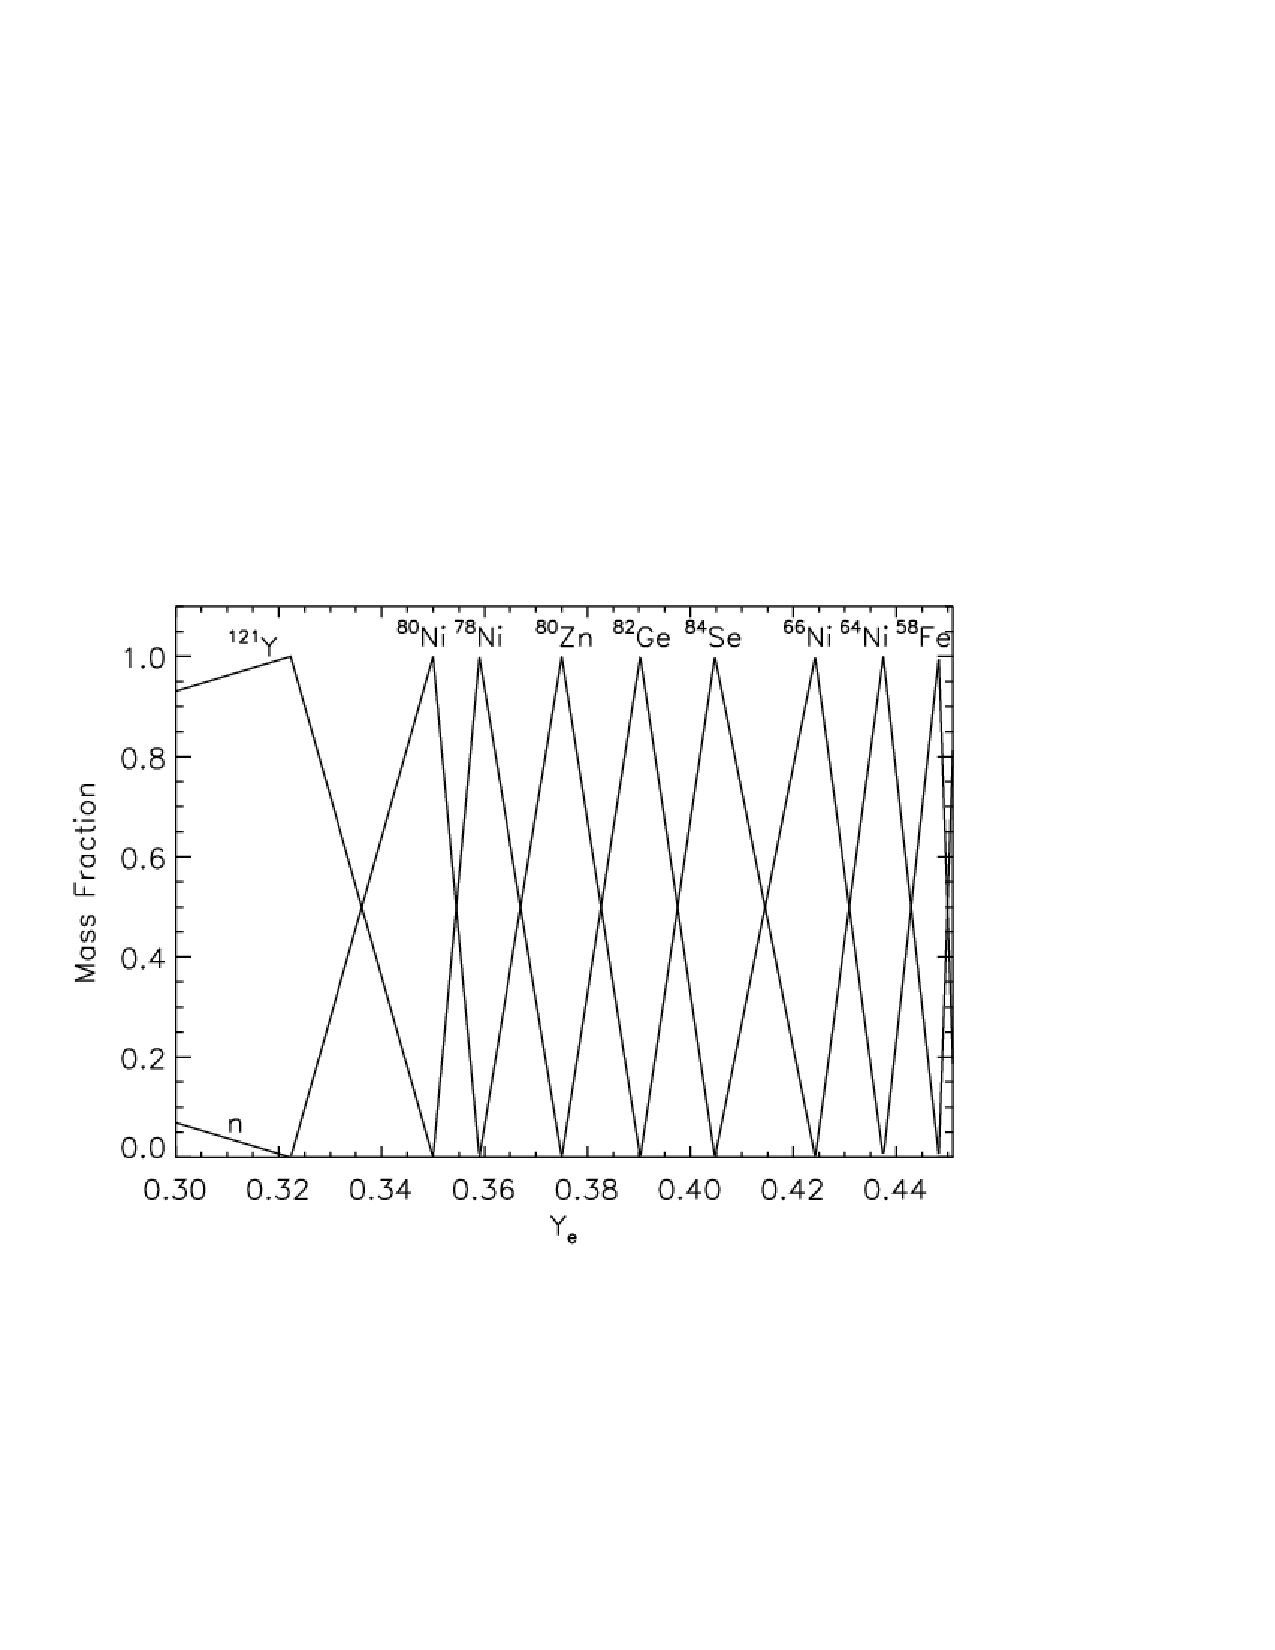
\includegraphics[width=5in]{figures/lower}
\caption{Mass fractions in a two-species, low temperature nuclear
  statistical equilibrium.}
\label{fig:lower}
\end{figure}

\begin{figure}[htp]
\centering
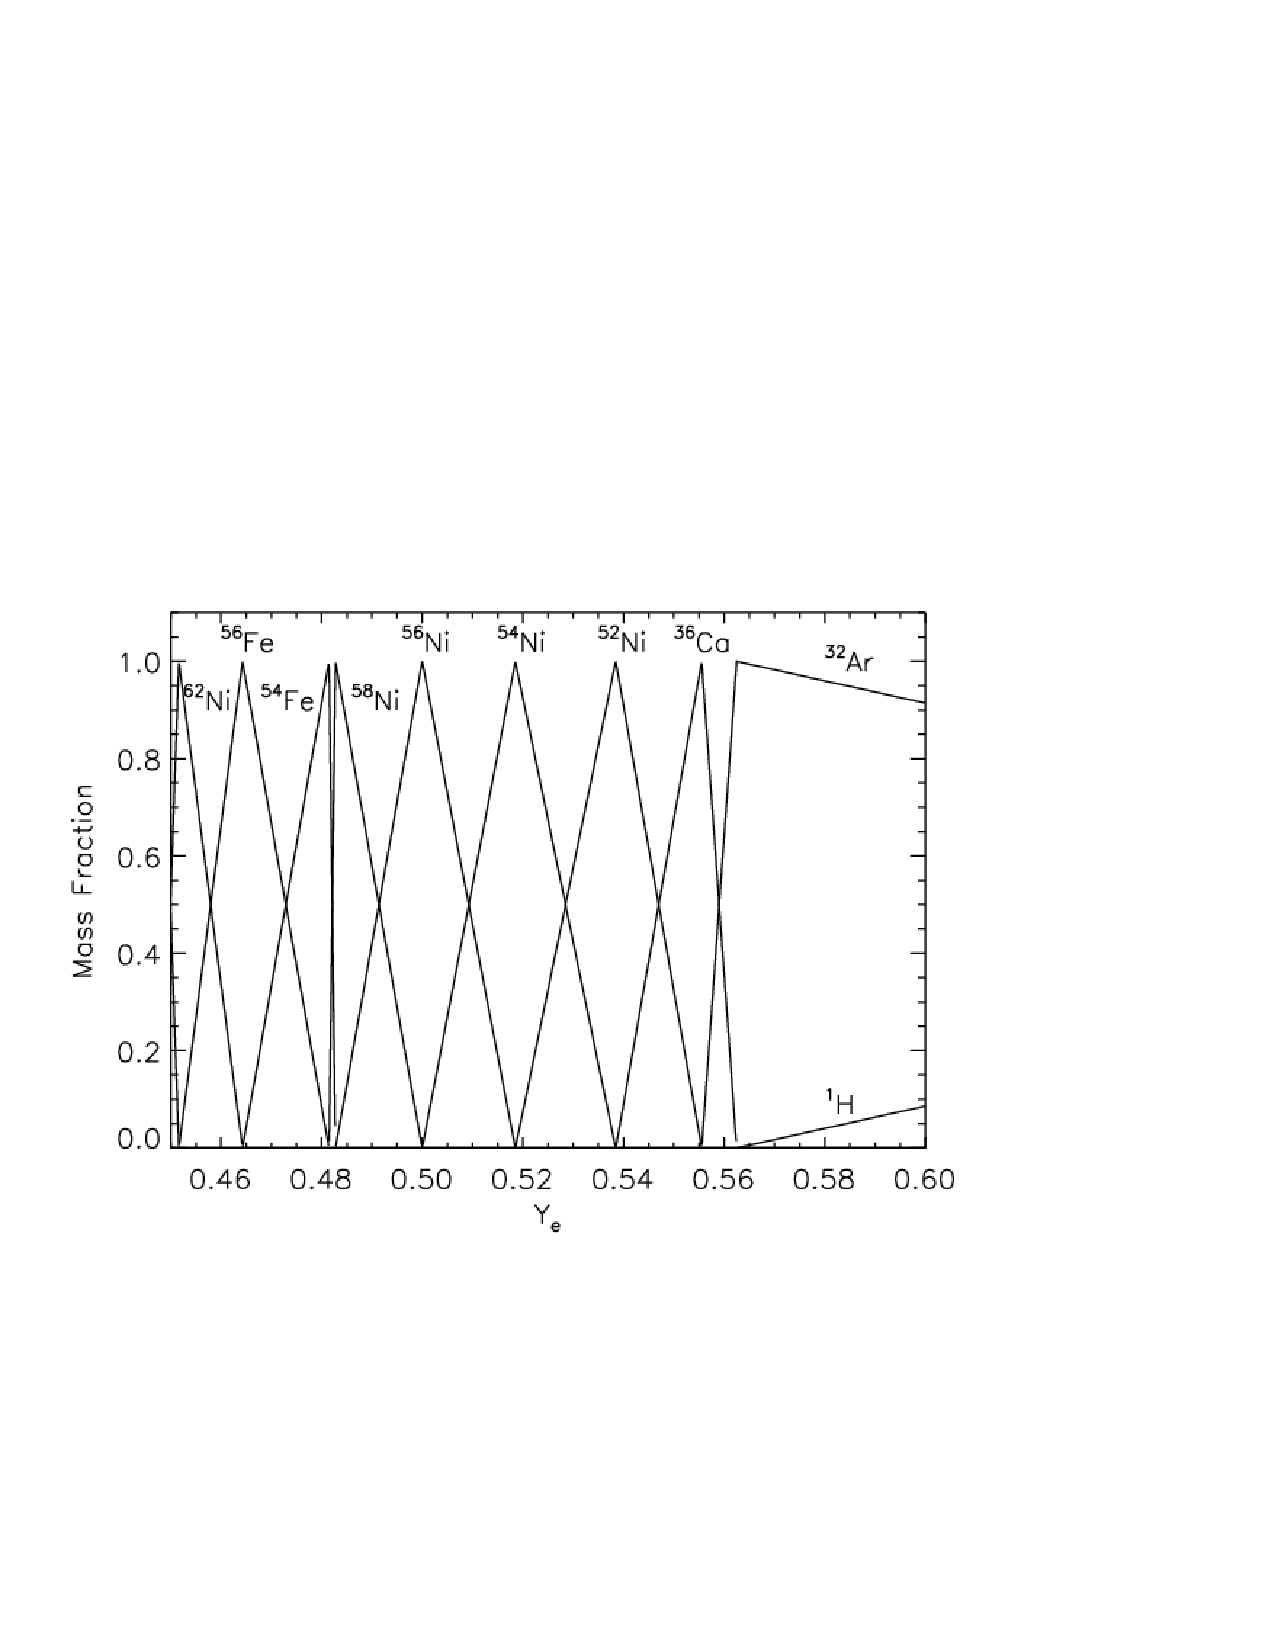
\includegraphics[width=5in]{figures/upper}
\caption{Mass fractions in a two-species, low temperature nuclear
  statistical equilibrium.}
\label{fig:upper}
\end{figure}

Figures \ref{fig:lower} and \ref{fig:upper} show the mass fractions that
satisfy Eq. (\ref{eq:f_2species}) for the mass file that comes with the
libnuceq 0.1 distribution.  At $Y_e = 0$, the system consists of
only free neutrons.  As $Y_e$ increases, the system becomes a mix of
free neutrons and $^{121}$Y.  As $Y_e$ increases further, the nuclei are
able to lock up all the neutrons, and the system is dominated by a mix
of various species (mostly in the iron group).  At certain values of $Y_e$,
the abundances are dominated by a single species with a $Z/A$ ratio equal
to the $Y_e$ value.  As $Y_e$ increases to values greater than 0.56, the
nuclei are not proton-rich enough to lock up all the protons, and the system
becomes a mix of $^1$H and $^{32}$Ar.  $^{32}$Ar is the winner for very
proton-rich nuclear statistical equilibria because, although it does not
have a particularly large binding energy per nucleon, it is a
particularly proton-rich species and can have a large abundance in proton-rich
environments.  Because it is bound, locking protons up into it reduces the
overall nuclear mass per nucleon in the system, thereby reducing the free
energy.  At $Y_e = 1$, the system, of course, consists only of free protons.

\begin{figure}[htp]
\centering
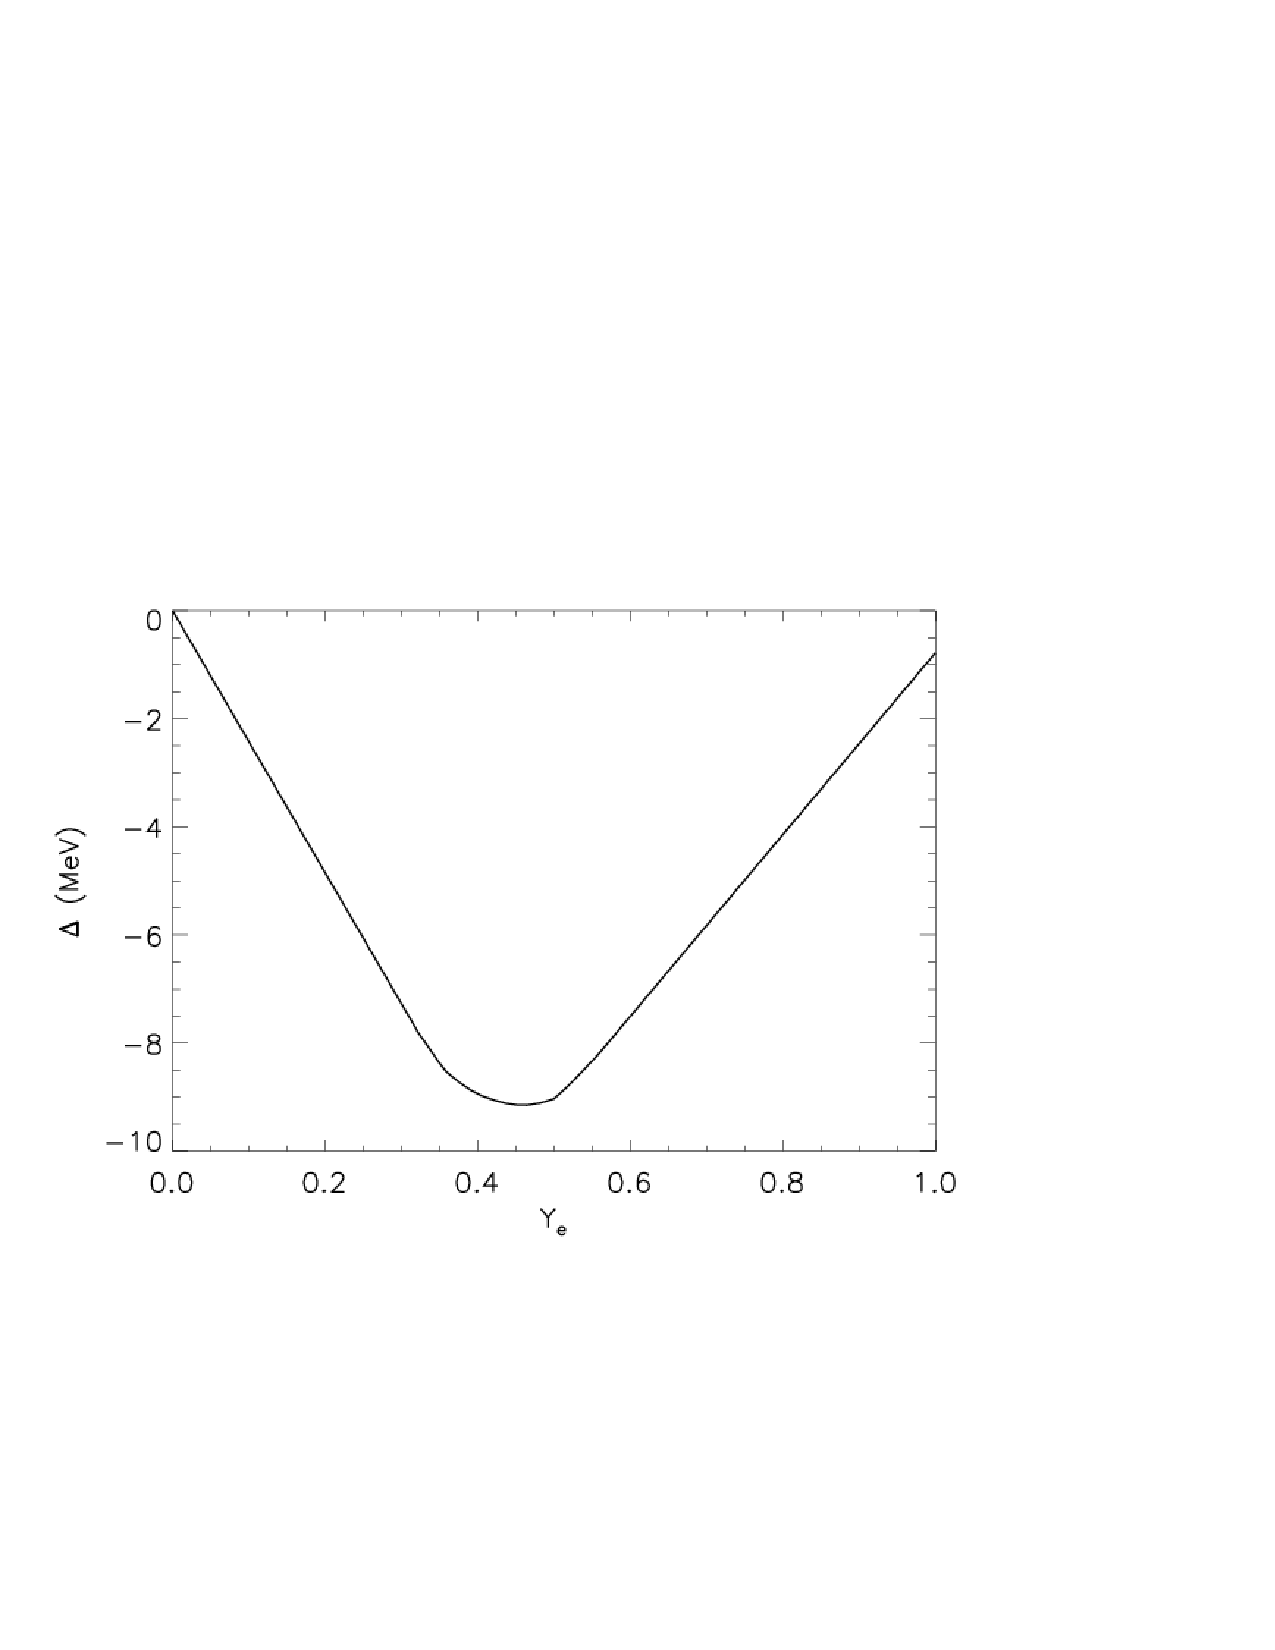
\includegraphics[width=5in]{figures/fig1}
\caption{Atomic rest mass per nucleon relative to the neutron rest mass in a
two-species low-temperature nuclear statistical equilibrium.}
\label{fig:fig1}
\end{figure}

\begin{figure}[htp]
\centering
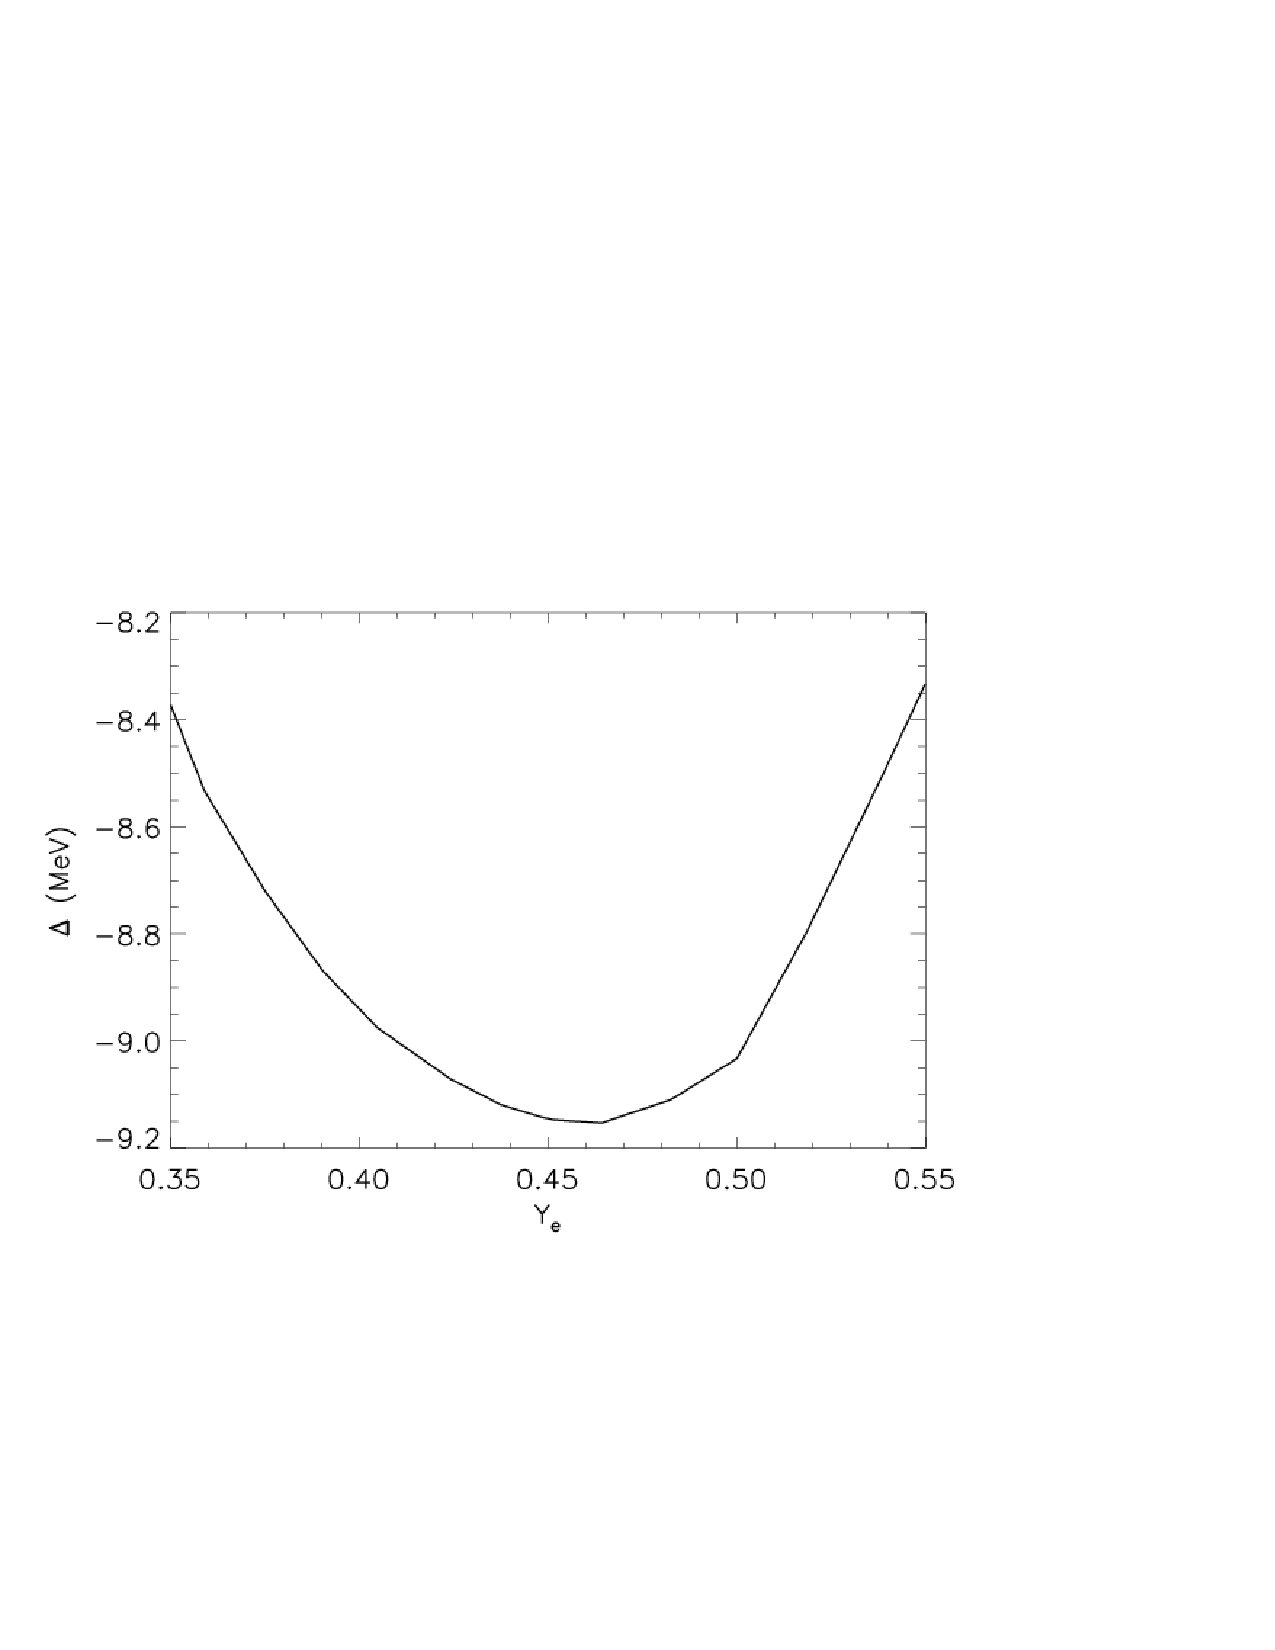
\includegraphics[width=5in]{figures/fig2}
\caption{Atomic rest mass per nucleon relative to the neutron rest mass in a
two-species low-temperature nuclear statistical equilibrium.}
\label{fig:fig2}
\end{figure}

Figure \ref{fig:fig1} shows the atomic mass per nucleon
relative to the neutron mass as a function of $Y_e$.  Figure \ref{fig:fig2}
shows the same curve but on a more restricted range in $Y_e$.  The
sudden breaks in the slope of the curve in Figure \ref{fig:fig2} are real
and are due to the sudden compositional changes evident in Figures
\ref{fig:lower} and \ref{fig:upper}.  The minimum atomic
mass per nucleon occurs at the $Y_e$ corresponding to $^{56}$Fe.  Thus,
the low-temperature system considered here would tend to evolve by weak
interactions until it consisted entirely of electrons and $^{56}$Fe.
This is somewhat surprising, given that $^{56}$Fe is not the nuclear
species with the largest nuclear binding per nucleon--$^{62}$Ni is.  The
reason $^{56}$Fe dominates is due to the fact that protons are less
massive than neutrons, and the lower mass from the
larger number of protons in the system dominated by $^{56}$Fe more
than compensates the tighter binding in the system dominated by
$^{62}$Ni.

\section{Low Temperature Calculations with libnuceq}

At low temperatures, libnuceq codes will calculate the correct nuclear
statistical equilibrium, as determined by the above considerations.
The difficulty will be that the accuracy of the abundances will not be
good due to the extremely large absolute values of the neutron and
proton chemical potentials.  Recall that the abundance of species $i$
in the equilibrium depends on the exponential of the quantity
$Z_i \frac{\mu_p}{kT} + \left(A_i - Z_i\right) \frac{\mu_n}{kT}$.
Numerical inaccuracies in the chemical potentials then propagate into
the abundances.

Another problem occurs for low temperature calculations of weak nuclear
statistical equilibrium.  At low temperatures, the electron chemical potential
can become extremely large during the root-finding iterations and the
default calculation of the electron number density fails.

The above problems occur for extremely low temperatures (tens of Kelvins
or less), which are not generally relevant to nuclear statistical equilibria of
physical interest.  At such low temperatures, one must consider that
the system may not be a plasma and the classical expressions for nuclei
are not relevant (the nuclei may become boson condensates!).  Should the
user be interested is very low temperature equilibria, he or she could extend
the considerations in \S \ref{sec:two_species}.  libnuceq-based codes should
be able to handle most other cases.

\end{document}
